\chapitre{Sanglots sur une vie brisée, le 27 juillet 2033 }{Tout ce qu’on fait dans la vie, même l’amour,}{ on le fait dans le train express qui roule vers la mort», avait écrit en 1928 l’artiste controversé Jean Cocteau lors d’une cure de désintoxication. Puisqu’il fumait de l’opium pour pouvoir «quitter le train en marche» et s’occuper d’autre chose que de la vie et de la mort, il n’avait pas encore réalisé qu’avec les années, le train devenait fou de vitesse, ivre de regret et prisonnier de ses rails, qu’il devenait de plus en plus infernal, fonçant dans un «voyage au bout de la nuit», celui de l’absurdité et de la pourriture dépeintes quelques années plus tard par Louis-Ferdinand Céline. Inexorablement, kilomètre par kilomètre, keclic-keclac, keclic-keclac, keclic-keclac, l’éclairage disparaissait, ce qui amenait le passager, de plus en plus apeuré, à vouloir mettre sa vie en lumière, comme pour se rassurer, à donner un sens à son errance, comme s’il eut fallu qu’il y en est un.  }

Et il s’y acharnait avant que la loco, celle de High Noon, le film culte de Fred Zinnemann, en vienne à siffler ses trois dernières prises, celles d’un arrêt sans buffet, sans gare, sans soleil, sans rien, le laissant abandonné, trahi, oublié, devant les forces obscures. «Trois prises ! Reeeetiréééé !» 

La Maririou qui ne dispose ni du surréalisme multidisciplinaire de Cocteau, ni de l’anarchisme cynique de Céline, ni de l’antimaccarthysme romantique de Zinnemann, vient de débarquer du train, attirée comme un papillon nocturne par une soudaine lueur dans le noir de la lumière disparue, lueur aussi blafarde que merveilleuse d’une allumette tenue à bout de bras par Marceline des Bezo. En râlotant, soufflant, chuintant, elle s’active devant Béatrice, Romain et Timothée, tous trois mis en sentiment par la chanson thème «Et toi aussi tu m’abandonnes», à déboulonner avec une clé à molette aussi longue que son archet, le sens qu’avait sa vie, celui dont l’épicentre était régi par les conventions musicales. Non pas pour redonner un sens au parcours accompli, tout le monde s’en fiche, y compris elle, mais plutôt pour aller, de ses pas précipités de petite vieille armée d’un parapluie, prendre le contrôle de la locomotive et donner cours à cette urgence de dire ce qui aurait dû l’être bien des années avant. Cocteau, Céline et Zinnemann n’avaient pu imaginer en leur époque qu’un jour, il y aurait la mentalité baby-boomer.

D’un ton sans appel, d’une voix définitive, elle raconte avoir passé sa vie à prétendre être musicienne violoncelliste, alors qu’elle ne l’était pas. Elle déclare n’avoir fait que besogner, gratter, peiner, triturer, sept jours sur sept, par temps de soleil, de grippe, de vide, pour en arriver à devenir une «bonne technicienne en manipulation de violoncelle». Eut-elle été musicienne violoncelliste, eut-elle été artiste, elle aurait été à l’écoute de la sensibilité des autres. Il aurait été naturel pour elle de vouloir l’enrichir, la nuancer, la soutenir, la compléter. Elle aurait su comment, et à quelle dose, ajouter sa petite particularité à elle dans l’émotion collective d’un ensemble musical. Mais non, elle ne vivait que pour ces œuvres où le violoncelle semble prendre toute la place, ces pièces magnifiques de Fauré, ces sonates et autre Allegro appassionato de Saint-Saëns, de Debussy, de Chopin, de Mendelssohn ou de Schubert, ces concertos pour violoncelle de Dvořák, de Boccherini, de Beethoven ou de Brahms. Et quand elle pouvait attirer tous les éclairages sur elle, quitte à laisser ses camarades dans le noir, elle le faisait du mieux qu’elle le pouvait. Ainsi, sous son archet, les deux concertos pour violoncelle de Chostakovitch devenaient des joyaux de perfection technique donnant droit aux vivats de la salle. Hélas!, insiste la Maririou, ce n’était que l’expression d’une habileté particulière, la prestation égotique d’une prouesse sans âme.

- Mon âme était rechtée dans le coffre d’une Impala rouge.

Incapable de remettre les pieds dans l’univers Bezo après le drame, Marie est allée vivre chez la cousine Lise à Rimouski, puis chez sa tante Denise à Québec; une petite boulotte toute gentille et sans enfants. Fortement repliée sur elle-même, parlant à peine à la sœur cadette de sa mère et presque jamais à son oncle Robert, un bon diable de plombier ronchonneur, la gamine s’est vite isolée dans sa chambre, on aurait dit une sauvageonne qui n’avait pas appris à sourire. Elle s’est raccrochée à la musique avec le gros crincrin du cousin Lucien, un «prêt à très long terme, ma chouette», et a choisi de ne pas fréquenter d’amis. De toute façon, elle n’en avait jamais eus.

Étonné par ses progrès plus que rapides à l’instrument, le couple de braves gens se met en tête d’inscrire la petite à des cours privés. C’est ainsi qu’un soir après souper, Denise l’amène dans le quartier Saint-Jean-Baptiste chez Michaela Prochazka, une violoncelliste tchécoslovaque qui s’était expatriée en 1945 juste avant que ne se referme l’étau soviétique. Entre 1938 à 1945, la dame avait joué avec l’Orchestre philharmonique tchèque, une formation très réputée qu’avaient naguère dirigée Antonín Dvořák, Gustav Mahler et Václav Talich.

- J’me chouviens des photos qu’elle m’a montrées. Tout était vrai; elle n’avait rien inventé. Mon Dieu que j’étais imprechionnée. Imaginez : être dirigée par Václav Talich !

À 82 ans, Marie se rappelle sans hésitation des noms de Michaela Prochazka et de Václav Talich. Elle n’a pas oublié, non plus, le fils de Mme Prochazka, ce petit salopard de Lukas. Elle revoit le salon de ce rez-de-chaussée, rue d’Aiguillon. Elle se remémore parfaitement bien le jour où sa professeure lui avait permis d’essayer son merveilleux instrument, une vénérable antiquité achetée à Belgrade dans les années 20.

- Je pense que chette femme m’a aimée.

Aimée, il faut le croire, puisque Robert Bérubé, qui s’était mis à son compte deux ans plus tôt, fait faillite en 1967. Le couple doit déménager dans un logement de Saint-François-d’Assise et se retrouve en situation de ne plus pouvoir supporter les cours privés. Heureusement pour la gamine, il n’est pas question de la retourner chez sa mère dans le Bas-du-Fleuve. «Y a des maudites limites à la misére», affirme Robert, l’œil humide. Apprenant la nouvelle, Mme Prochazka offre sans aucune hésitation, un peu comme si elle choisissait une partition, de continuer à enseigner gracieusement, ce qu’elle fera avec le plus grand sérieux jusqu’à l’admission de Marie au Conservatoire de musique de Québec.

- À chette époque, mon oncle Robert dijait que les doigts de ma main gauche étaient tellement forts que les jommes avaient peur de moi. T’as jamais eu peur que j’te torde le cou, Romain ?

- Non parce que j’ai toujours eu le cou plus gros que ta main. Mais ta langue, par exemple, ouf !

Sa formation a eu comme cadre unique la ville de Québec où tout se termine en 1972 avec un Premier Prix du Conservatoire de musique de Québec en violoncelle, ce qui lui permet de faire quelques remplacements à l’Orchestre symphonique de Québec et à la Société de musique contemporaine du Québec. Mais, ambitieuse insatiable, elle veut fréquenter la célèbre Juilliard School de New York, une perspective nettement au-dessus de ses moyens. D’où la France, pays avec plein de gens cultivés où, assurément, il est possible de gagner sa vie avec un violoncelle, là-bas, et même de se ramasser un pactole, ce qui contribuera à se payer la Juilliard. Une semaine après être débarquée, elle signe un contrat avec l’Orchestre philharmonique Rhône-Alpes à Lyon, emploi qu’elle s’était déniché directement de Québec, ce qui lui permet de s’acheter un instrument fabriqué à Mirecourt au début du XXe siècle. 

\begin{floatingfigure}[l]{45mm}
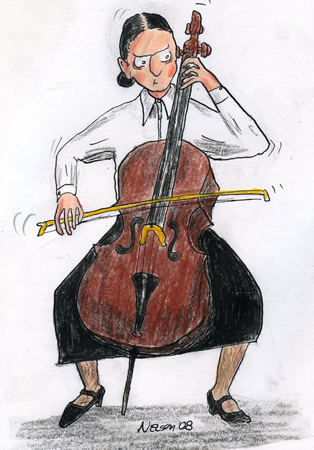
\includegraphics[height=60mm]{corps/chapitre16/img/personnage-marie-musique.jpg}
\end{floatingfigure}

Pendant huit ans, elle arpente ainsi les coins et recoins de l’Hexagone et, à bien y penser, en déborde à plusieurs reprises. Par contre, elle doit faire son deuil des grands orchestres symphoniques, ceux de Berlin, de Munich, de Londres. Quand elle tente sa chance auprès de l’Orchestre symphonique de Navarre Pablo Sarasate, l’humiliation qu’elle en ressent lui sert une leçon qu’elle méditera toute sa vie : connaître sa force, savoir quelle est sa place et ne jamais «péter plus haut qu’le trou !»

Pendant huit ans, Marie Rioux se tire d’affaire avec d’excellentes formations, quoique de moindres envergures, tels l’Orchestre symphonique de Tours, l’Orchestre Symphonique Municipal de la Ville de Nice ou l’Orchestre du Capitole de Toulouse et elle a collaboré avec de très jeunes ensembles dont l’Orchestre national de Lille ou L’Orchestre national d’Île de France. Elle travaille également avec de plus petits groupes, dont à Bernes et à Genève avec un quatuor à cordes, à Marseille et à Lyon avec un orchestre de chambre. Mais surtout elle tyrannise pendant deux ans, la douzaine de valeureux musiciens de l’Orchestre de Chambre de Toulouse. C’est que partout, la «fille à Marceline» se retrouve en situation de coups et blessures. On la déteste uniformément : violoniste qui se fait détruire sa tenue de concert, une autre qui découvre ses partitions dans une cuvette souillée, violoncelliste concurrente à qui elle cache une importante pratique, altercation en plein récital dans un musée bernois, volée d’injures en français bas-laurentien envoyée à un maestro de son âge, un Danois qu’elle jugeait obnubilé par son ego, et ainsi de suite.

1 mètre 80, svelte, élégante, normalement vêtue de noir, le port altier, le visage très beau bien que fermé, les yeux de la couleur du fleuve lors des grandes marées d’automne quand il arrache tout son fond pour en faire une bouillie qu’il recrache sur ses berges, Marie subit régulièrement des tentatives masculines de rapprochement, des manœuvres libidineuses à peine masquées, des passes grossières de drague, voire quelques propositions directes qu’elle reçoit comme des soufflets. Elle arrive toujours à tout repousser. Même Arnaud Muller, virtuose de la flûte traversière, qui l’aime à en vouloir mourir. Il est prêt à tout abandonner pour elle, dont sa femme et sa fillette. Quand la violoncelliste apprend ce détail en dînant dans un quatre fourchettes de Grenoble, elle fait un tel esclandre, incluant son Côte du Rhône dont elle asperge la figure du malheureux, que l’amoureux éconduit quitte l’orchestre, défait, découragé, misérable.

Côté disque, elle n’en aura jamais un à son nom, contrairement à ce que colportera, par après, la rumeur culturelle de la région rimouskoise. Par contre, en tant que musicienne dans une formation, elle va participer à plusieurs reprises à des enregistrements, des initiatives qui la laisseront de glace, mais qui la frustreront à l’occasion, surtout quand elle ne pourra s’agiter les crins que sur quelques portées. Ce que l’on grave, déplorera-t-elle, semble toujours être conçu pour mettre n’importe quel instrument en valeur, sauf le violoncelle.

Tant et si bien qu’à la fin de l’hiver de 1980 Marie Rioux, à la veille d’avoir 29 ans, est devenue une boule de nerfs prête à exploser. Vierge, solitaire, isolée, crainte, détestée, désillusionnée, mauvaise, crevée morte, elle va consulter un médecin toulousain qui lui colle un diagnostic de surmenage professionnel, ce syndrome d’épuisement dont la médecine faisait alors de plus en plus de cas.

- Il faut arrêter quelque temps, ma p’tite dame. Sinon, crac, ça sera la camisole !

- Me semble qu’avec un p’tit remontant, je passerais à travers, non ?

- Plaît-il ?

- Z’avez pas des pilules qui me tireraient d’affaire ?

- Je vous parle de votre vie et vous me causez de «pilules». Soyez sérieuse, il vous faut vous soigner.

- Me soigner …

- Vous reposer, ma p’tite dame, seulement vous reposer, sans rien faire d’autre. Je veux bien vous prescrire des cachets, mais seul le repos pourra vous amener à un complet rétablissement.

La jeune femme repart avec, en poche, une prescription appréciable et la justification médicale d’un arrêt de travail. Comme elle est sur le point de partir en tournée avec l’Orchestre de Chambre de Toulouse, aussi bien en Espagne, au Canada, qu’aux É.-U., elle s’entend pour être remplacée le plus tôt possible et, coïncidence, le nouveau violoncelliste est attendu après la prestation de Québec, la quatrième au Canada.

C’est un concert de musique baroque, essentiellement du Mozart, qui, en ce beau dimanche après-midi de printemps, a pour cadre le Musée de Québec, sur les Plaines d’Abraham. Tout au long, Marie y bouge son archet comme si elle était zombie. Ce qu’a bien sûr remarqué Rhéa Théberge, l’institutrice du 2e Rang Ouest de Saint-Fabien, qui est assise dans la salle, son programme utilisé comme éventail. Le récital terminé, elle s’approche de la pièce où sont passés les musiciens et demande qu’on avertisse Marie Rioux de sa présence.

- Tu n’as presque pas changé depuis la dernière fois que je t’ai vue; c’était à Rimouski. Tu es seulement plus grande et plus jolie.

Marie reconnaît cette femme qui l’a initiée à la lecture, à la musique, à la connaissance, cette femme qui a catalysé sa sortie d’un milieu malsain.

- Mamzelle Théberge ?

- Oui ma belle, c’est moi, de répondre l’enseignante devenue quadragénaire avancée, en embrassant généreusement son ancienne pupille.

Cernée, les traits tirés, amaigrie, la musicienne explique sa situation. C’est son dernier concert; on l’a mise au repos et elle en a au moins jusqu’à l’automne, si ce n’est plus. Après ? Elle ne le sait trop. Peut-être rappliquera-t-elle en France reprendre le collier. Elle est sous contrat avec l’Orchestre de Chambre de Toulouse, une chic organisation dont elle ne veut surtout pas abuser; elle leur en a assez fait subir. Elle est aussi en sabbatique avec l’Orchestre du Capitole de Toulouse, mais n’a vraiment pas envie d’y retourner. Peut-être ira-t-elle plutôt étudier à New York. Pour l’instant, elle est sous l’effet des médicaments et ne veut plus penser à rien. Non elle n’a pas de mari ou d’ami de cœur et cela est bien loin de ses préoccupations. En fait, elle n’a ni chat, ni chien, ni canari, ni plante, ni maison. Elle n’a qu’un petit studio qu’on ne lui loue pas cher, rue de Mirepoix, un «chouette quartier à deux pas de la Garonne».

- T’es quasiment rendue avec un accent français ?

- Ça se corrige !

- La Garonne, chanceuse !

Marie frise le début de sourire.

- Ouais. La Garonne, c’n’est peut-être pas un vrai bras de mer, un vrai fleuve salé comme le nôtre, mais c’est un cours d’eau qui a son charme.

À son tour, Rhéa raconte qu’elle a abandonné sa petite école depuis belle lurette; en fait, il n’en existe plus d’écoles de rang. Les citadins les ont achetées. Ils en ont fait des maisons, des chalets. Non, depuis quelques années, elle s’occupe passionnément de jeunes en difficulté, de cas complexes issus de familles dysfonctionnelles, monoparentales, miséreuses, de victimes de violence, des enfants parfois traumatisés pour le restant de leurs jours. Tous souffrent d’un énorme problème d’image, d’absence de perspective leur permettant de voir qu’ils pourraient peut-être s’en tirer. Et en les parquant dans une même école, dans une même classe, la commission scolaire les a ghettoïsés. Autour d’eux, ils ne voient que malheur, échec, pauvreté et médiocrité. Sans compter qu’ils sont discriminés et ridiculisés par toutes les autres classes.

- Mais toi, Marie, tu représentes tout le contraire. Tu t’en es sortie. En dix-huit ans, tu es passée de la misère noire du 3e Rang Ouest à un studio près de la Garonne. Tu voyages, tu donnes des concerts et tu gagnes très bien ta vie. Et en Europe par-dessus le marché ! Et si je me fie à ce qui est en vente à la sortie de la salle ici, tu joues dans des 33 tours. Ça, moi, j’appelle ça réussir sa vie de façon extraordinaire.

La jeune femme commence à vouloir filer; elle perçoit très bien où cette conversation s’en va.

- Je vais être bien honnête avec toi. Je suis venue pour te demander une faveur.

- Vous voulez que j’aille rencontrer vos enfants, que je leur prouve qu’on peut s’en sortir, que dans le fond, un père qui nous bat, une mère qui nous boit des verres de gin sous le nez, c’est grave, mais que le fait de cesser de rêver qu’on va s’en sortir, l’est encore plus ? C’est ça ?

- À peu près ça, oui.

- Oubliez ça, mamzelle Théberge, j’en suis incapable. J’ai de la misère à vivoter dans mon petit monde à moi, un petit monde gros comme ça dans ma pauvre caboche. J’ne commencerai pas à aller le présenter à d’autres en le quittant temporairement pour pouvoir entrer dans le leur. J’n’en suis pas capable. Vraiment pas. Il est faux de croire, mamzelle Théberge, que je m’en suis sortie ! À force de ne pas savoir comment inventer la machine à remonter le temps qui me permettrait d’aller rescénariser mon enfance, je suis devenue une garce invivable que tout le monde déteste. Et faut absolument que je me repose !

C’est à ce moment que la quémandeuse sort l’arme-choc de sa besace. Hypocritement, elle lui parle d’une petite fille de 11 ans, sa copie carbone, 18 ans en arrière, une enfant perdue, recluse, fermée, incapable de sourire, jamais d’amis, battue et laissée pour compte par une monoparentale toxicomane de Rimouski-Est. La totale !

Dans la tête de Marie, deux fils oubliés viennent se toucher et toute son expression change. La perfide Rhéa a gagné !

Quelques jours plus tard, la musicienne est debout devant une classe en apparence normale. On a beau voir à leurs vêtements que les deux douzaines d’enfants sagement assis ne sont pas riches, rien n’indique qu’ils sont des pestiférés normatifs. Si certains semblent enchantés de rencontrer cette co-miséreuse d’une autre époque, la plupart l’écoutent avec de grands yeux gênés. Mais tout au fond, physiquement en retrait, une petite fille, probablement de onze ans, fait semblant, du mieux qu’elle le peut, de ne pas l’entendre ni la regarder.

- Comment t’appelles-tu ? lui demande Marie.

- A parle pas, madame, crie un gamin. Elle s’appelle Sonia Gagné.

Dès lors, la jeune femme n’a d’yeux que pour cette fillette. Elle ne semble plus parler qu’à elle. Même que le soir, invitée à coucher chez Rhéa, une sorte de commémoration des occasions où il ne faisait pas beau dans le rang, elle questionne abondamment son hôte sur la petite Sonia. Elle veut tout savoir. On la dirait fascinée. Dans sa tête, une mission surgit : sauver cette enfant. Elle doit le faire. Ce n’est pas pour rien que le destin les a mises en présence, toutes les deux.

Le lendemain matin, avant de s’en retourner au terminus d’autobus, elle demande au chauffeur de taxi de l’amener à un magasin de musique où elle achète un harmonica. De là, elle passe à l’école, donne le petit instrument au secrétariat afin qu’on le remette, de sa part, à Sonia Gagné et file vers son car.

- Là, cha va aller vite, continue La Maririou. Ma tante Denije à Québec avait un cougin qui louait des chalets au lac Chaint-Mathieu. Le mois chuivant, je l’ai appelé et il m’a organigé quek’chose de pas pire, achez proche du lac et achez loin des gens.

Pendant les deux dernières semaines de juin, la convalescente séjourne au lac où elle se divertit à chasser les écureuils, les ratons laveurs et les oiseaux qui viennent les importuner, elle et son violoncelle, dans les innombrables pièces de ce château qu’elle a tôt fait de se construire dans son monde imaginaire, un monde salutaire qu’elle avait toujours eu le loisir de rendre totalement étanche aux réalités qui, ça et là, l’agressaient. Une irrépressible impulsion l’amène cependant à prendre régulièrement des nouvelles de la petite Sonia. Oui elle s’amuse avec son harmonica. Non elle ne s’est pas informée sur sa bienfaitrice. Oui elle a terminé ses classes. Non elle ne sera pas promue au degré supérieur.

L’avant-veille de son départ pour Québec, elle apprend de Rhéa la création de l’École populaire de Musique, un projet communautaire du milieu où il est question d’initier des enfants et des adultes défavorisés aux joies de la musique par l’apprentissage d’un instrument. Elle a pris sur elle d’y inscrire Sonia en violon…

- T’as dix-huit ans de violoncelle dans le corps, ma belle, tu dois bien savoir jouer du violon, non ?

C’était en effet un instrument que Marie maniait avec une certaine dextérité, mais une dextérité ampoulée, rigide, classique et fort peu violoneuse.

- J’te dis ça d’même parce qu’il y a eu trop d’inscriptions en violon; ils manquent de profs.

Comme elle tourne en rond, qu’elle ne sait trop quoi faire de ses 10 doigts, qu’elle n’a vraiment pas envie de s’installer chez sa tante Denise, qu’elle a suffisamment d’épargne pour se permettre de ne pas travailler pour presque un an, qu’il pourrait être judicieux de se changer un peu les idées et que, dans le fond, elle pourrait aider la petite Sonia à s’en sortir, la jeune femme demande à l’enseignante de venir la chercher. Elle rencontrera les autorités du projet.

Le responsable de l’enseignement, Pierre Dugrain, est un professeur de violon au conservatoire local qui se met à saliver devant le CV que la violoncelliste lui dépose sur la table du bar où il la reçoit sans cérémonie.

- Premier prix en violoncelle, Orchestre Symphonique de Tours, Orchestre Symphonique de Nice, Orchestre du Capitole de Toulouse, Orchestre national de Lille, Orchestre national d’Île de France, Orchestre de Chambre de Toulouse, barnak, t’en a fait du millage ! Maudit beau CV !

Marie se fait prudente.

- Je suis violoncelliste, pas violoniste.

- Barnak, c’t’une job de bénévole qu’on t’offre. On rentrera pas la Guilde des musiciens dans notre affaire, casse-toi pas la tête ! Par contre, continue Dugrain, je sais qu’au Conservatoire, on a besoin d’un chargé de cours en violoncelle pour septembre. Si ça t’intéresse, va appliquer. Avec un CV comme le tien, t’es certaine d’avoir la job. Pis là, b’en c’est pas du travail bénévole. Tu veux une bière ?

- Merci, j’bois jamais d’alcool, qu’elle répond avec douleur, revoyant les caisses honnies que son père vidait à l’époque.

Ici, raconte la mère de Timothée, il y a tout un paradoxe à expliquer. D’une part, elle devient très rapidement «la Maririou», un personnage austère, exigeant, autoritaire que collègues et étudiants adorent détester. Ainsi, dès le départ, elle fait croisade contre le fait que la gestion d’un si beau projet avait été confiée à une clique de noceurs, incluant Dugrain, qui tenaient l’essentiel de leurs réunions décisionnelles dans une buvette aussi malfamée qu’enfumée du centre-ville de Rimouski. Pour elle, une telle pratique était illégale, inefficace et non respectueuse auprès des membres de l’équipe qui ne fumaient pas, ne prenaient pas de drogue et ne consommaient pas d’alcool, dont elle était probablement la seule représentante. Elle en fait tant, qu’elle se retrouve isolée et tournée en dérision. Marie se replie donc, coupe tout contact non essentiel et demande à ce qu’on ne lui affecte plus que des moins de douze ans, les plus mal en point, insiste-t-elle, ce qui, bien sûr, inclut Sonia Gagné. Encore là, sa nature conflictuelle prend le dessus. Des enfants se plaignent, d’autres se présentent de plus en plus rarement. Seuls les plus timides semblent se résigner à continuer. Quant à Sonia, elle finit par réagir en abandonnant définitivement ses cours. Elle conserve toutefois l’harmonica.

- Je l’ai jamais revu ch’te pauvre p’tite fille-là. Chi elle est encore vivante, elle doit bien avoir proche 65 ans. Timothée est à veille d’la voir entrer au Chentre !

D’autre part, elle subit humiliation sur humiliation, accepte le sobriquet de Maririou, continue de donner toutes les heures qu’on lui demande, essaie par tous les moyens de mettre de l’eau dans son vin pour que les petits démunis qu’on lui envoie ne souffrent pas trop. Elle devient la personne la plus fiable de l’École et même Dugrain est obligé de le reconnaître, lui qui doit, par ailleurs, s’immiscer dans une jacquerie d’étudiants du Conservatoire incapables de supporter l’extrême rigueur de la chargée de cours. Malgré tout, elle demeure fidèle à ses engagements de l’été 80. Jamais elle ne fléchira. On dira d’elle qu’elle est «le roc sur lequel l’École a été bâtie». En fait, elle négociera avec les édiles de son village pour que de façon nominale, l’École puisse louer une ancienne maison bourgeoise saisie pour taxes non payées. Grâce à une armée de bénévoles et de donateurs, le bâtiment sera rénové et adapté aux besoins de l’enseignement musical, cela sous la supervision constante et méticuleuse de la Maririou.

- Mais j’ai fini par m’adouchir avec le temps, dijons que je me chuis calmée. Je pense que ch’est Romain qui a eu le dechus. 

\begin{floatingfigure}[l]{40mm}
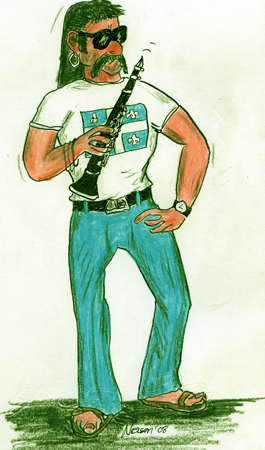
\includegraphics[height=60mm]{corps/chapitre16/img/personnage-romain-jeune.jpg}
\end{floatingfigure}

Romain, le beau clarinettiste autodidacte qui lui a vraiment fait basculer sa vie ! Il lui a essentiellement démontré qu’elle ne comprenait rien à la musique. Pour elle, c’était un travail douloureux qu’il lui fallait accomplir à la perfection, une peine quotidienne, constante, truffée d’exigences pas possibles, un délire exutoire que l’on devait présenter à des gens ayant payé et devant applaudir. C’était accepter des conditions scandaleuses pour plaire à de rondouillets bourgeois ravis, repus, roteux. C’était consacrer sa vie à se battre entre collègues pour une petite place dans un ensemble que viendra peut-être entendre le politicien, le financier, le m’as-tu-vu, des salauds sans sensibilité artistique qui auront une influence sur la survie financière de la formation musicale. C’était traîner son étui à violoncelle d’orchestre en orchestre pour appuyer la tendance voulant que la musique soit une business faisant surtout vivre des gens, analphabètes devant une partition, mais très habiles en marketing et en relations publiques. Or, a répété Romain autant de fois qu’il l’a pu, la musique ne peut être qu’un plaisir constant, qu’une joie solitaire pouvant évoluer en trip entre copains, en concerts gratuits dans des endroits sympathiques, en jam-sessions entre instrumentistes et autres tapeurs de pieds.

- La musique, on la fait pour soi, pour se faire plaisir, pour se faire du bien. On joue de la musique. On apprend aux autres à jouer, pas à suer !

Toute une conception, tout un projet de société ! Quoi qu’il en soit, le gaillard lui a fait découvrir une planète qu’elle ignorait. Partie toute jeune d’un environnement miséreux, elle a vécu chez des gens modestes de Québec, puis s’est acclimatée au sud de la France sans fréquenter personne. La voici maintenant dans un monde de marginaux qui s’aménagent d’impressionnants jardins engraissés au capelan, qui s’essaient dans l’élevage de petites chèvres, de lapins et de volaille, qui produisent des variétés touchantes de confitures, de gelées, de ketchup, de conserves, qui confectionnent eux-mêmes leurs rideaux, leurs carpettes, leurs couvre-lits, qui n’ont jamais moins de cinq chats et deux chiens, des énormes, qui conduisent des camionnettes rafistolées et qui, avec respect, s’établissent dans des villages traditionnels. Un univers de filles en robes longues, bottées comme pour faire le train, sans jamais de soutien-gorge et qui se roulent leurs cigarettes, de gars qui ne se taillent plus la barbe, qui ne portent que des bottes «capées», qui achètent leur Dow en caisse de 24 petites ou de 12 grosses et qui se disent en accord avec les revendications féministes.

Eux, Marie et Romain, ils s’installent au sortir de Saint-Anaclet, sur les hauteurs de Rimouski, dans une maison épouvantablement maganée dont le terrain d’une dizaine d’acres pourrait devenir intéressant. Or, contre toute probabilité, ils vont y demeurer 47 ans. Grâce à Romain, la jeune femme apprend à vraiment sentir une fleur, à bien observer un bourdon, à mâchouiller et déguster un brin de foin, à jouer avec une portée de chats, à batifoler nue dans certaines anses du Bic, à fréquenter les gens sans leur arracher les yeux, à boire des grosses bières, à ne pas se laver tous les jours et surtout, à jardiner. Marie se découvre en effet le pouce vert.

Dès l’automne, elle sait qu’elle ne regagnera pas l’Europe. Là-bas, personne ne la manque et aucun ensemble ne lui fait parvenir d’offre d’emploi. C’est aussi à ce moment qu’elle devient convaincue que sa sexualité est «foquée». Elle ne peut commettre l’acte que gelée. Alors, elle peut ressentir un certain plaisir et parfois, du désir. Autrement, rien n’est plus désagréable, voire irritant. Faut-il préciser qu’elle ne met pas grand temps à adopter la béatitude des drogues douces, ce qui l’amène à connaître l’essentiel état de détente qui lui avait fait défaut jusque-là. Quant à son mauvais garçon d’amoureux, il s’ouvre à la discipline des partitions musicales, ce qui lui permet d’acquérir un peu de rigueur, qualité dont il était cruellement dépourvu.

Pendant les dix premières années, ils vivent d’expédients, d’aventures, de trafics dérisoires et de miracles. Chaque année, la Maririou chasse son beau Romain et, à chaque fois, elle le regrette. Sur une base irrégulière, elle enseigne à des jeunes dans le cadre du projet et, contre rémunération, ses économies ayant été dissipées, à des étudiants du conservatoire. De temps en temps, il arrivera une petite fille de onze ans toute poquée que Marie essaiera d’initier à la musique. Parfois, ça semblera vouloir fonctionner pour quelque temps, parfois ça ne lèvera pas. C’est dire les frustrations de cette nouvelle Michaela Prochazka qui veut à tout prix aider ces victimes d’un émule d’Edmond Rioux.

Il en est ainsi jusqu’en 1990 quand, à 39 ans, elle donne naissance à Timothée-Milet. Tout change alors. Vraiment. Romain embrigade ses deux frères, des Longueuillois, dans une offensive majeure au terme de laquelle un banquier lui consent l’hypothèque nécessaire à l’achat de cette brinquebalante maison qu’ils louent depuis les débuts à Saint-Anaclet. Au printemps suivant, il accepte même ce travail de livreur en fourgonnette que lui propose un voisin, l’homme d’affaires Gilles Lévesque. Dès lors, il coupe radicalement dans sa consommation de hash et se résout, sans bougonner, à se taper toutes les heures supplémentaires qu’on lui impose. C’est ce cabotage routier qu’il fera sur les routes locales et régionales pendant les trente prochaines années, sans jamais déplaire. De son côté, Marie ramasse tous les cours qu’on lui confie et se met à produire des confitures, des conserves et des fines herbes qu’elle vend dans un petit stand que lui aménage Romain près du chemin devant leur maison.

- À partir de là, cha va être la routine et le temps va filer.

Romain veut nuancer.

- T’oublies le lac Saint-Mathieu. On y a loué une roulotte à tous les étés …

- On l’a fait entre 1997 et 2015, deux chemaines par été.

Le lac Saint-Mathieu, ce sera leurs vacances annuelles. Marie réussira à combiner ce court séjour avec un mini camp musical où certains enfants seront conviés aux frais de l’École. Sans s’occuper de cette marmaille dans le quotidien, elle supervisera individuellement leur pratique instrumentale. Eh oui, Timothée, il y a eu la petite Julie, cette nièce catégorie fesse gauche de Luce Morency, une fillette qui lui semblait vraiment intéressée à se donner à la musique, à fuir son univers sordide, une petite fille très sensible qu’en cet été 2001, elle a rapidement aimée et placée au centre de ses préoccupations quotidiennes.

- On l’a retrouvée battue à mort en janvier 2010. Elle était gelée comme une crotte, plantée dans un banc de neige comme un piquet à côté du prechbytère d’Amqui. On n’a jamais chu ch’qui ch’était passé. Cha m’a fait de la peine, pauv’ ‘tite fille !

À deux occasions, la Maririou va s’impliquer en politique, une fois localement, une autre, au niveau du comté. En 2014, des édiles municipaux veulent mettre la main sur la bâtisse louée un dollar par année à l’École de Musique quinze ans plus tôt. Ils ont beau jeu, la paperasse semble avoir été un peu bâclée à l’époque. Leur projet ? Raser l’équipement et récupérer le terrain pour agrandir le mini mail voisin. La perspective étant jugée inacceptable, Marie s’en va-t’en-guerre, fait du porte-à-porte et se fait élire conseillère. C’est ainsi qu’elle va arriver à tout bloquer. À la table du Conseil, elle va devenir une mère chat à qui de méchants roquets de perron veulent enlever ses chatons. La bataille sera terrible et, au terme, les promoteurs devront baisser pavillon ayant épuisé toutes leurs ressources et leur patience. Presque vingt ans plus tard, on en parle encore.

En 2019, un courant de pensée visant à sabrer les dépenses culturelles sévit, encore une fois, à la grandeur du Québec. Ainsi, la survie de l’École est en jeu. À 68 ans, Marie va aller cogner chez Sylvain Turcotte, un fils de cultivateur qui a été désigné comme nouveau candidat libéral pour le comté de Rimouski. Méticuleusement, comme s’il s’agissait de l’enjeu politique le plus important de la planète, elle lui expose toute la problématique et le convainc d’intégrer la survie de l’École dans sa plate-forme électorale. En contrepartie, elle accepte de l’appuyer publiquement, elle la grande musicienne qui a endisqué, qui a joué partout, cette vedette internationale qui a amassé tous les prix et qui est respectée par tous les chefs d’orchestre au monde. En outre, elle décide de travailler lourdement à son élection. Il est important de souligner que cette fois, la Maririou n’est pas, comme à son habitude, le pire des fléaux. De nombreux bénévoles libéraux attribuent cette dignité à Mimi Turcotte, directrice adjointe de l’organisation libérale pour le comté de Rimouski et mère du candidat. Il va de soi que Marie se découvre ici un alter ego, une femme aussi tête de nœud qu’elle-même pouvait l’être. On connaît la suite, le gros Turcotte, élu haut la main grâce à un taux de participation de plus de 45 %, sera nommé ministre et, malgré ses promesses maintes fois répétées de soutenir l’École envers et contre tous, il ne lèvera pas son auriculaire boudiné pour la protéger quand, deux ans plus tard, elle devra fermer définitivement ses portes faute de pouvoir se financer adéquatement. C’est une disparition qui affectera profondément Marie; il n’y aura plus jamais de petites filles de 11 ans à tenter de sortir de la misère.

Lorsqu’en 2021, Romain va décider qu’il en a assez et qu’il prend sa retraite – il est âgé de 70 ans - la vie du couple va, dès lors, devenir plus difficile. Les piges au conservatoire seront de plus en plus rares et le jardin de plus en plus ténu.

- Ch’est pour cha que j’ai tellement pouché fort pour que tu acchepte le contrat sur la Côte-Nord avec Jérôme Dubé.

Romain se garde bien de répondre. Il lorgne plutôt Gazou qui dort, son horrible tête dans ses petites pattes crochues. Marie boit une gorgée d’eau avant de conclure.

- Cha été cha, ma vie !

Une vie où, insiste-t-elle, elle est passée à côté de l’essentiel, non pas sa carrière musicale, mais la vraie vie. Elle a vécu 70 ans convaincue que sa mère ne l’avait pas aimée, qu’elle ne l’avait pas défendue, qu’elle avait tué Edmond, ce père monstrueux, pour se défendre, elle, bien après que son enfant eut été battue sans qu’elle ne lève le petit doigt. Par la suite, Marie a passé sa vie à craindre les hommes, particulièrement ceux qui avaient de grosses paluches, «pas de belles mains de clarinettichte comme Romain», ceux qui parlaient fort, ceux qui voulaient décider pour les autres, ceux qui donnaient des ordres, «pas évident quand tu joues dans un orchechtre de chambre», ceux qui buvaient beaucoup.

Elle a imposé à son seul enfant et à son vieux compagnon des choix de vie qui ne leur convenait pas. Timothée, ce petit garçon rêveur, tendre, sensible, le cœur sur la main, elle l’a enfermé dans un enfer de musique-labeur, de respect de l’autorité, de crainte des femmes et de discipline incessante, cela par crainte qu’il ne ressemble à son grand-père Rioux, alors qu’il n’en avait pas du tout le caractère, contrairement à elle, Marie, qui en avait hérité quelques grands pans. Romain, ce vrai artiste, cette si bonne nature, cet homme de cœur et de vérité, elle l’a enferré dans une vie sérieuse, besogneuse, gratteuse, dangereuse et pire encore, alors que si elle l’avait laissé faire, leur vie aurait tellement été meilleure.

Elle cesse de contempler le tapis pour regarder son compagnon.

- Il y a 6 ans, je t’ai forcé à gâcher ce qui te restait de vie et par ricochet, chelle de Timothée ! Je m’en veux, tellement, tellement …

Elle a tenté d’aider de petites victimes à se sortir de leur misère en leur présentant une merveilleuse porte de sortie, mais aucune n’a voulu la suivre. Elle a cru que si la musique avait été la panacée dans son cas, il se pouvait qu’elle le soit dans leur cas. Mais était-ce bien une panacée ? Avec le recul, elle comprend maintenant – maintenant qu’il est trop tard - qu’elle n’a fait, à onze ans, que changer de cage et de système de valeurs. Elle sait aujourd’hui que la musique n’a jamais été une vocation, mais un refuge. Car, isolée dans le 3e Ouest de Saint-Fabien ou isolée dans sa musique, c’est, dans les deux cas, être coupée de la réalité. Comment, alors, peut-on faire en sorte que de petites filles toutes brisées en viennent à se raboudiner juste assez pour s’engager dans la vraie vie sur leurs deux pattes ?

- Je t’ai jamais remerchié, Romain, pour m’avoir montré che qu’étais la vraie réalité. J’aurais donc dû !

Un silence pesant succède au long récit. Timothée sait que s’il essaie de parler, rien ne sortira. N’a-t-il pas suffisamment étalé la preuve de sa désorganisation émotive ? Le vieillard, lui, a baissé la tête. Il vient de recevoir un premier remerciement en 53 ans de vie commune et ne sait trop quoi en faire. Sa réaction ne pourra qu’être brouillonne. Quant à Béatrice, elle arrive à bien mesurer toute l’intensité du moment et sent l’émotion lui agacer la luette.

C’est alors que pour la première fois depuis 1962, Marie Rioux, enfant battue de onze ans qui semble, cette fois, avoir abandonné la douce protection de son monde imaginaire, une cosmogonie complexe si loin de la vraie réalité, celle des petites filles qu’on retrouve mortes à Amqui dans un banc de neige, Marie Rioux descendue de son train sous les regards empathiques de ses proches, éclate en sanglots. C’est un pleur fait de hoquets lents, creux, typiques aux gens qui sans avoir désappris à pleurer, s’y remettent à l’étonnement général. Elle tente de se contrôler, de reprendre contenance, mais en vain. Elle essaie de parler, mais sa bouche ne lui obéit plus comme il le faudrait. Trop de peine doit en sortir.

- J’ai tout raté, parvient-elle quand même à exprimer, sans réaliser qu’à l’aide de son parapluie en canne, elle était en train de grimper dans une locomotive. Je vous demande même pas de me pardonner, il est trop tard pour cha. J’ai 82 ans et chuis enfermée dans un chous-chol.

La séquence est insoutenable. Alors que Romain et Timothée sont figés, Béatrice bouleversée par une telle expression de détresse, s’approche du fauteuil et se penche vers Marie pour l’enserrer dans ses bras. Doucement, elle lui caresse les cheveux.

Gazou que la scène a dérangé se rassure en apercevant la belle dame étreindre sa maîtresse. Il branle de la queue un instant et se replonge dans son sommeil.